\problemname{Meeting Place}
$N$ friends live on each vertex in a tree with $N$ vertices, where $N$ is an \textbf{odd} number.
A \emph{tree} is a connected graph with exactly $N-1$ edges.

The friends want to meet at one vertex in the tree.
They have agreed that the best meeting place is the vertex that minimizes
the sum of distances to the friends, and have asked you to help them find 
this optimal meeting place.
The \emph{distance} $\text{dist}(a,b)$ between two vertices $a$ and $b$ in the tree is 
the number of edges on the path between $a$ and $b$.
So formally, the goal is to find the vertex $x$ that minimizes 
$\sum_{i=1}^{n} \text{dist}(x,i)$.

You think this is an easy problem, and start writing a solution right away.
But there is a twist!
The friends have bad memory and don't remember what the tree looks like.
However, they do remember the following: given three \textbf{different} friends 
$a,b,c$, they can tell you the vertex where those three usually meet, which is
the vertex $x$ that minimizes
$\text{dist}(x,a) +\text{dist}(x,b) +\text{dist}(x,c)$.
Note that $x$ is not necessarily one of the vertices $a$, $b$ or $c$.

In this problem you will not read the graph from the input, instead you can ask $Q-1$
questions on the form:
\emph{Where do the friends $a,b,c$ usually meet?}
Your task is to find the optimal meeting place by using these questions.

\begin{figure}[!h]
\begin{center}
  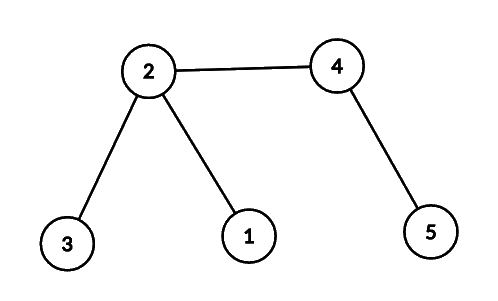
\includegraphics[width=7cm]{sample.png}
\end{center}
  \caption{The tree in the sample. Vertex 2 is the optimal meeting place.}
\end{figure}

\section*{Interaction}

The first line of input contains two integers $N$ and $Q$,
the number of vertices in the tree, and the number of queries you can make.
It is guaranteed that $N$ is odd and that $Q = 500\,000$ in all test cases.

Then you can make the following queries:
\begin{itemize}
  \item Output one line with ``\verb|? a b c|'' where $1\le a,b,c\le N$ are $3$ \textbf{different} friends.
    After that, the judge will respond with one integer $x$ that you should read from input
    ($1\le x\le N$), the vertex that minimizes $\text{dist}(x,a) +\text{dist}(x,b) +\text{dist}(x,c)$.
  \item Output one line with ``\verb|! x|'' where $1\le x\le N$ is the optimal meeting place.
    After you have printed this query your program should terminate without outputting anything more. 
    If $x$ is the vertex that minimizes $\sum_{i=1}^{n} \text{dist}(x,i)$ you will get \textit{Accepted} on the test case, otherwise you will get \textit{Wrong Answer}.
\end{itemize}
If you make more than $Q$ queries (including the last on the form ``\verb|! x|'')
your program will be terminated and you will get \textit{Wrong Answer}.

\textbf{Make sure to flush the output after each query}, otherwise you may get \textit{Time Limit Exceeded}.
In C++ this can be done for example with \texttt{cout << flush}
or \texttt{fflush(stdout)};
in Python with \texttt{stdout.flush()};
and in Java with \texttt{System.out.flush()}.

\section*{Scoring}
Your solution will be tested on a set of test case groups.
To get points for a group, you must pass all test cases in the group.


\noindent
\begin{tabular}{| l | l | l |}
  \hline
  Group & Points & Constraints \\ \hline
  $1$   & $10$        & $3 \le N\le 99$ and all vertices have degree at most 2 (the tree is a line) \\ \hline
  $2$   & $12$        & $3 \le N\le 999$ and all vertices have degree at most 2 (the tree is a line) \\ \hline
  $3$   & $21$        & $3 \le N\le 24\,999$ and all vertices have degree at most 2 (the tree is a line) \\ \hline \hline
  $4$   & $14$        & $3 \le N\le 99$ \\ \hline
  $5$   & $15$        & $3 \le N\le 999$ \\ \hline
  $6$   & $28$        & $3 \le N\le 24\,999$ \\ \hline
\end{tabular}
